\section{Pan-Tilt}

Para el control de la orientación de una cámara en este proyecto, se utiliza un sistema Pan-Tilt. Este mecanismo permite ajustar con precisión la dirección en la que la cámara está orientada, ampliando el campo de visión y mejorando la versatilidad del sistema. Los movimientos del sistema Pan-Tilt son controlados a través del microcontrolador ESP32, que gestiona las órdenes provenientes de la interfaz de usuario.



El Pan-Tilt utilizado está construido de forma artesanal y se encontraba en el laboratorio del departamento. Se construyó para un artículo científico llamado en inglés ``A new approach in controlling the motors of a binocular camera head'' \cite{PanTilt2004}. Se ha optado por su uso con la intención de mantener el sistema lo más abierto y adaptable posible.



Este mecanismo está equipado con servomotores HITEC HS-645MG\footnote{HITEC HS-645MG Datasheet \url{https://media.digikey.com/pdf/Data\%20Sheets/Hi-Tech/HS-645MG.pdf}}, que son reconocidos por su alta resistencia, robustez y precisión. Estos servomotores son capaces de mover y mantener de manera precisa la posición de la cámara, a pesar de las vibraciones o las cargas externas (véase la figura \ref{figure:pan-tilt})

\begin{figure}[!htb]
   \centering
    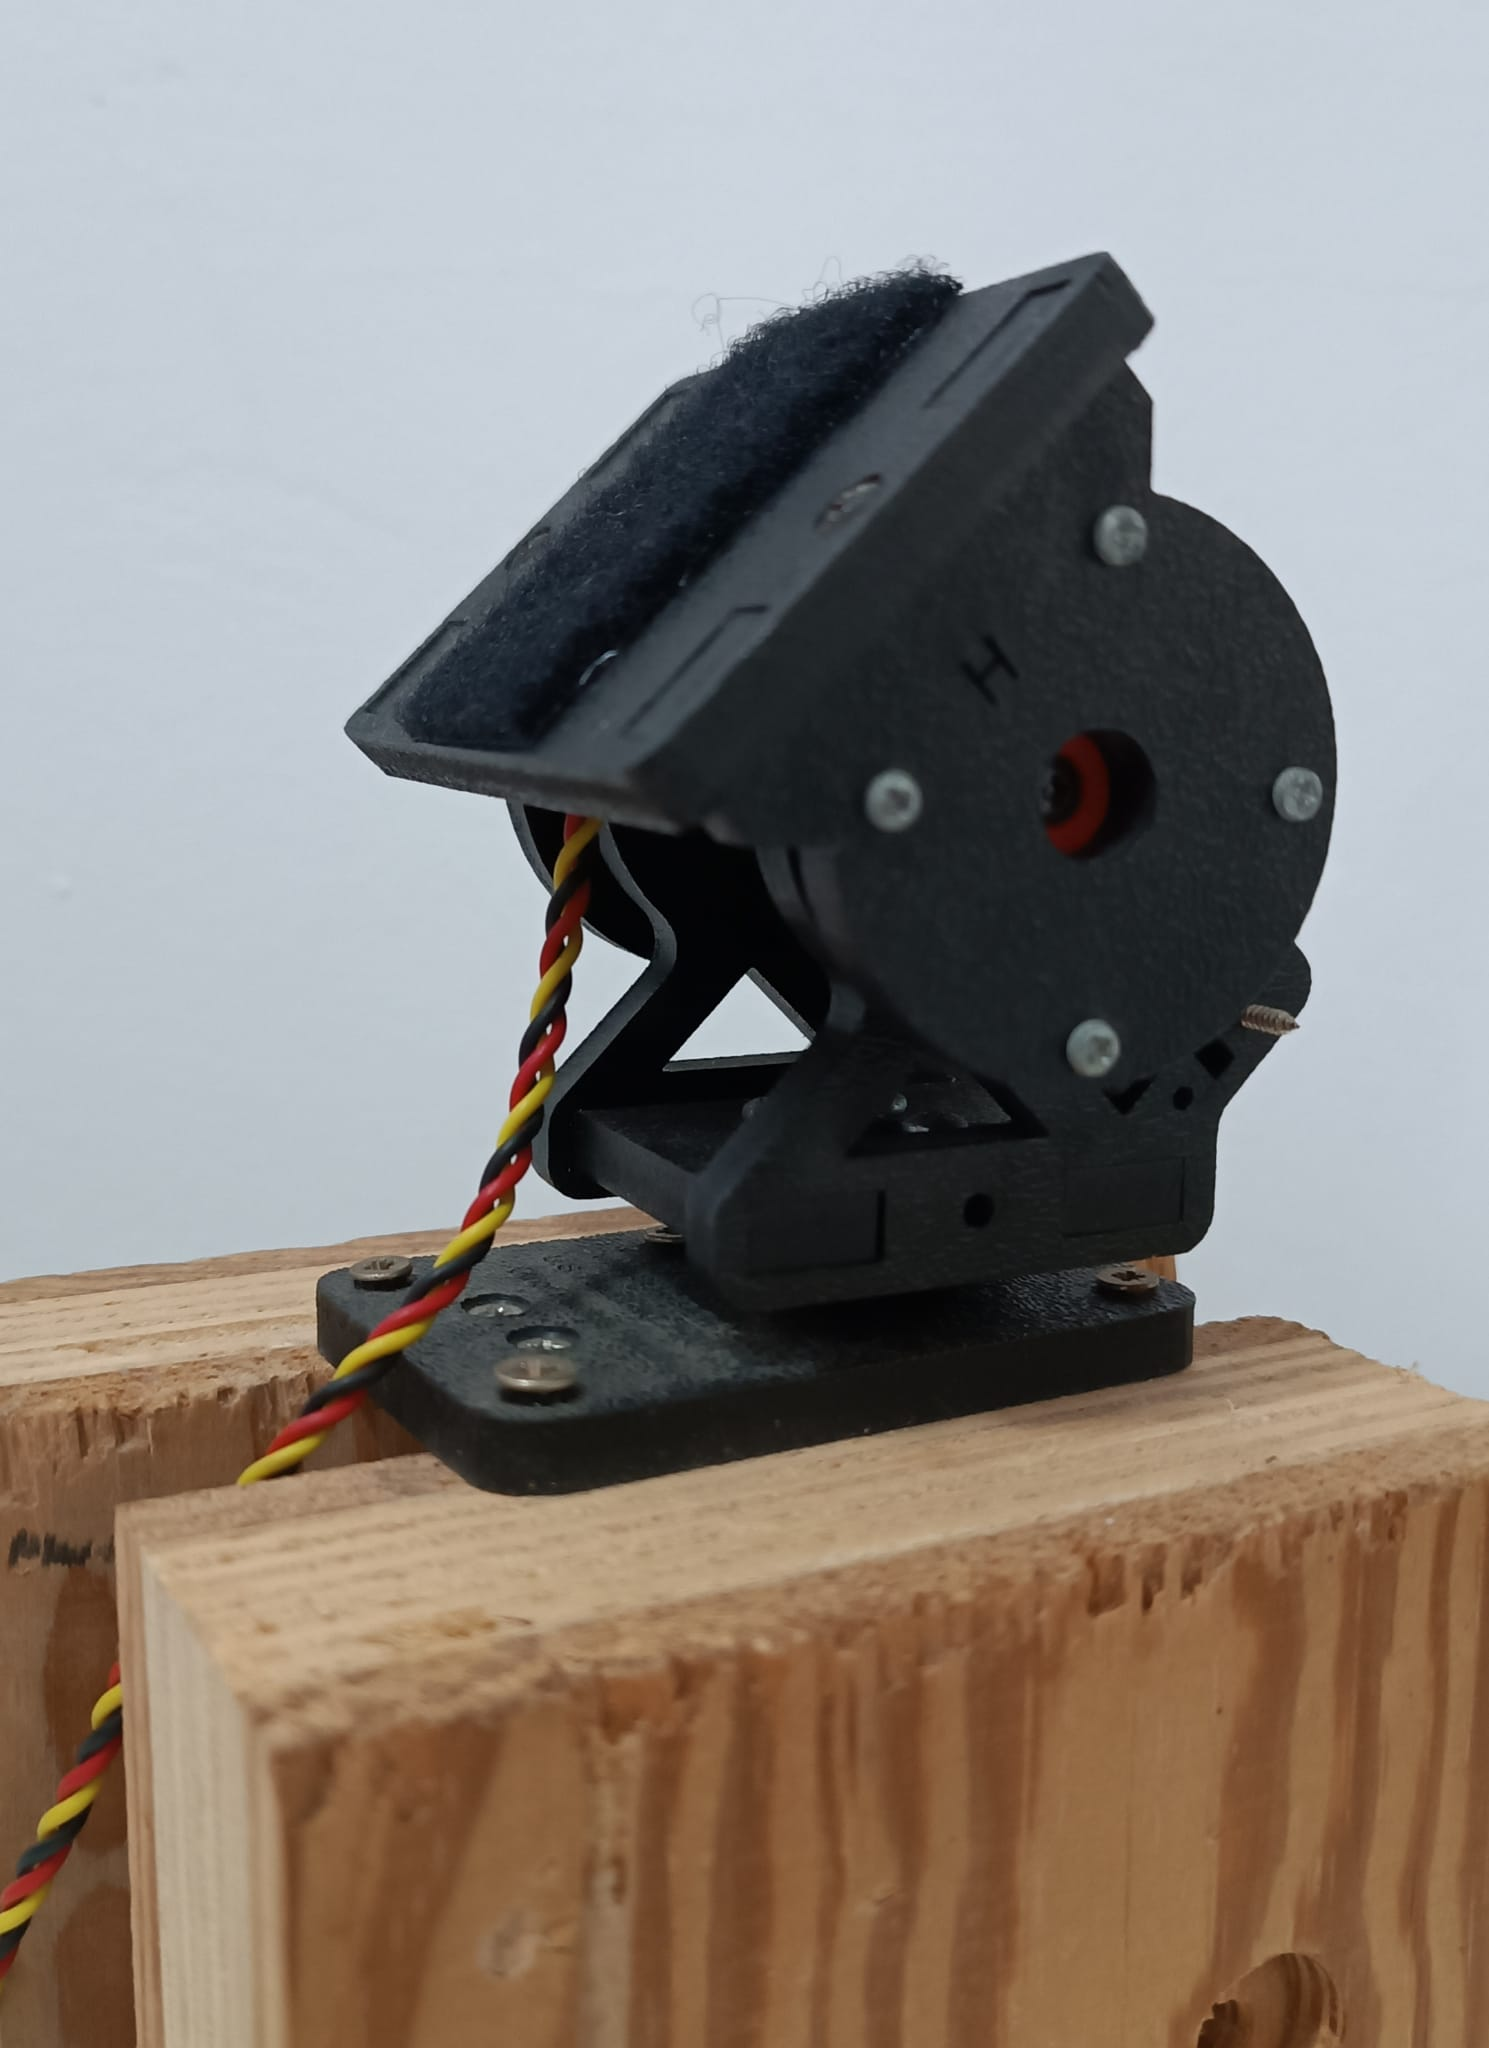
\includegraphics[width=0.3\linewidth]{figures/pan-tilt.jpg}
   \caption{Pan-Tilt artesanal}
   \label{figure:pan-tilt}
\end{figure}